\documentclass[12pt, a4paper, oneside]{ctexbook}
\usepackage{amsmath}
\usepackage{amsfonts}
\usepackage{mathabx}
\usepackage{subcaption} 
\usepackage{cancel}
\usepackage{pifont}
\usepackage{circledsteps}
\usepackage{bm}
\usepackage{tcolorbox}
\usepackage{amsthm,amsmath,amssymb}
\usepackage{floatrow}
\usepackage{caption}
\usepackage{geometry}
\usepackage{graphicx}
\usepackage{wrapfig}
\usepackage{mathtools}
\usepackage{scalerel}    
\usepackage{extarrows}
\usepackage{color,framed,hyperref,mathrsfs}

\title{{\Huge{\textbf{信息论}}}\\——笔记整理}
\author{BarryMafu}
\date{\today}
\linespread{1.5}
\newtheorem{theorem}{定理}[section]
\newtheorem{definition}[theorem]{定义}
\newtheorem{lemma}[theorem]{引理}
\newtheorem{corollary}[theorem]{推论}
\newtheorem{example}[theorem]{例}
\newtheorem{proposition}[theorem]{命题}
\newtheorem{exercise}[theorem]{练习}
\newenvironment{solution}
  {\renewcommand\qedsymbol{$\blacksquare$}\begin{proof}[解答]}
  {\end{proof}}

%----- 自定义命令 -----
\newcommand{\Z}{\mathbb{Z}}
\newcommand{\N}{\mathbb{N}}
\newcommand{\R}{\mathbb{R}}
\newcommand{\Q}{\mathbb{Q}}
\newcommand{\C}{\mathbb{C}}
\newcommand{\E}{\mathbb{E}}
\newcommand{\Pow}{\mathcal{P}}
\newcommand{\cov}{\mathsf{Cov}}
\newcommand{\var}{\mathsf{Var}}
\newcommand{\A}{\mathcal{A}}
\newcommand{\bA}{\boldsymbol{A}}
\newcommand{\ii}{\mathrm{i}\mkern1mu}
\newcommand{\abs}[1]{\left\vert#1\right\vert}
\newcommand{\norm}[1]{\left\lVert#1\right\rVert}
\newcommand{\dx}[1][x]{\mathop{}\!\mathrm{d}#1}
\newcommand{\del}[2]{\dfrac{\partial#1}{\partial#2}}
\newcommand{\red}[1]{\textcolor{red}{#1}}
\newcommand{\emp}[1]{\textcolor[RGB]{193, 0, 53}{#1}}
\newcommand{\sbe}{\ensuremath{\subseteq}}
\newcommand{\spe}{\ensuremath{\supseteq}}
\newcommand{\sbne}{\ensuremath{\subsetneq}}
\newcommand{\spne}{\ensuremath{\supsetneq}}
\newcommand{\Ord}{\ensuremath{\text{Ord}}}
\newcommand{\al}{\ensuremath{\alpha}}
\newcommand{\be}{\ensuremath{\beta}}
\newcommand{\ga}{\ensuremath{\gamma}}
\newcommand{\de}{\ensuremath{\delta}}
\newcommand{\te}{\ensuremath{\theta}}
\newcommand{\et}{\ensuremath{\eta}}
\newcommand{\ld}{\ensuremath{\lambda}}
\newcommand{\Al}{\ensuremath{\bm{\alpha}}}
\newcommand{\Be}{\ensuremath{\bm{\beta}}}
\newcommand{\Ga}{\ensuremath{\bm{\gamma}}}
\newcommand{\De}{\ensuremath{\bm{\delta}}}
\newcommand{\Te}{\ensuremath{\bm{\theta}}}
\newcommand{\Et}{\ensuremath{\bm{\eta}}}
\newcommand{\Xx}{\ensuremath{\bm{\xi}}}
\newcommand{\ci}{\ensuremath{\circ}}
\newcommand{\s}{\ensuremath{\ast}}
\newcommand{\ra}{\ensuremath{\rightarrow}}
\newcommand{\Ra}{\ensuremath{\Rightarrow}}
\newcommand{\la}{\ensuremath{\leftarrow}}
\newcommand{\La}{\ensuremath{\Leftarrow}}
\newcommand{\LR}{\ensuremath{\Leftrightarrow}}
\newcommand{\LLR}{\ensuremath{\Longleftrightarrow}}
\newcommand{\ora}[1]{\overrightarrow{#1}}
\newcommand{\ag}[1]{\langle#1\rangle}
\newcommand{\para}{\mathrel{/\negmedspace/}}
\newcommand{\bPhi}{\boldsymbol{\Phi}}
\newcommand{\bff}{\boldsymbol{f}}
\newcommand{\by}{\boldsymbol{y}}
\newcommand{\bc}{\boldsymbol{c}}
\newcommand{\bxi}{\boldsymbol{\xi}}
\newcommand{\bI}{\boldsymbol{I}}
\newcommand{\ca}[1]{\ensuremath{\mathcal{#1}}}
\newcommand{\bd}[1]{\ensuremath{\boldsymbol{#1}}}
\newcommand{\td}[1]{\ensuremath{\tilde{#1}}}
\newcommand{\bphi}{\boldsymbol{\phi}}
\newcommand{\vvector}[1]{\left(\begin{matrix} #1 \end{matrix}\right)}

\DeclareMathOperator*{\Span}{Span}
\DeclareMathOperator*{\im}{Im}
\DeclareMathOperator*{\rank}{rank}
\DeclareMathOperator*{\card}{card}
\DeclareMathOperator*{\grad}{grad}
\DeclareMathOperator*{\argmax}{argmax}
\DeclareMathOperator*{\epi}{epi}
\DeclareMathOperator*{\maximize}{maximize}
\DeclareMathOperator*{\minimize}{minimize}
\DeclareMathOperator*{\Null}{Null}
\DeclareMathOperator*{\CC}{CC}

\begin{document}

\maketitle

\pagenumbering{roman}
\setcounter{page}{1}

\begin{center}
    \Huge\textbf{前言}
\end{center}~\

2025秋季,王立威教授的机器学习课程。

\bigskip
仍在施工中,请带好安全头盔!
\begin{figure}[h]
    \centering
    
\includegraphics[width=.5\textwidth]{pic/pf-under_construction.png}
\end{figure}

~\\
\begin{flushright}
    \begin{tabular}{c}
        BarryMafu\\
        \today
    \end{tabular}
\end{flushright}

\newpage
\pagenumbering{Roman}
\setcounter{page}{1}
\tableofcontents
\newpage
\setcounter{page}{1}
\pagenumbering{arabic}

\chapter{集中不等式}

\section{前置数学知识}

在介绍不等式前,先回顾一些概念.以后会使用如下记号:
\begin{definition}
    对于命题(或随机变量)$u$,定义\textbf{示性函数}(indicator function)
    \[
    \mathbb{I}[u] = \begin{cases}
        1 &, u \ \text{成立} \\
        0 &, \text{否则}
    \end{cases}
    \]
\end{definition}

接下来,回顾一下概率论中的一些结论
\begin{theorem}(Markov不等式)
    随机变量$X$满足$X\ge 0$,且$\E[X] < \infty$,则对于任意$k \ge 0$,都有 
    \[
    \Pr[X \ge k] \le \dfrac{\E[X]}{k}
    \]
\end{theorem}
\begin{theorem}(Chebyshev不等式)
    随机变量$X$满足$\E[X] < \infty, \var(X) = \sigma^2$,则对于任意$k \ge 0$,都有 
    \[
    \Pr[\abs{X - \E[X]} \ge k] \le \dfrac{\sigma^2}{k^2}
    \]
\end{theorem}

布置了练习
\begin{exercise} \label{exr:taildistrib}
已知随机变量$X \sim \mathcal{N}(0, 1)$,定义 
\[
\Phi(t) := \Pr[X \ge t] = \dfrac{1}{\sqrt{2\pi}}\int_{t}^{+\infty} e^{-\tau^2/2} \dx[\tau]
\]
可以证明$\Phi$并不是初等函数,现求一个初等函数$f \sim \Phi$,即二者渐进等价。
\end{exercise}

\textbf{分析} \quad 先分析一下这个问题:显然$\Phi(t) \ra 0$,所以要$f \ra 0$. 现在$\Phi$的形式非初等不便于分析,不妨考虑$\Phi'(t) = \varphi(t)$,为此可以运用L'Hospital法则:
\[
\lim_{t \ra +\infty} \dfrac{\Phi(t)}{f(t)} = \lim_{t \ra +\infty} \dfrac{\Phi'(t)}{f'(t)} = \lim_{t \ra +\infty} \dfrac{-C e^{-t^2/2}}{f'(t)}
\]
其中$C$是某常数. 我们希望$f \sim \Phi$,也就是上述极限为1, 所以为了化简,我们希望$f'(t)$中也出现$e^{-t^2/2}$的形式. 回忆到 
\[
v(x)e^{u(x)} = \Big(v'(x) + u'(x)v(x) \Big) \cdot e^{u(x)}
\]
因此我们不妨设$f(t)$形如$g(t) e^{-t^2/2}$,此时
\[
\lim_{t \ra +\infty} \dfrac{-C e^{-t^2/2}}{f'(t)}
= \lim_{t \ra +\infty} \dfrac{-C e^{-t^2/2}}{\big[g'(t) - tg(t)\big] \cdot e^{-t^2/2}} = \lim_{t \ra +\infty}\dfrac{-C}{g'(t) - tg(t)}
\]
欲使上式为1,就要
\[
\lim_{t\ra +\infty}  tg(t) - g'(t) = \dfrac{1}{C}
\]
简便起见只考虑$C=1$,之后再给$g$乘上系数. 注意!这里千万不要把其当作$-g'(t) + tg(t) = 1$这样的一阶线性常微分方程求解,因为其解不保证初等. 如果你尝试求解ODE会发现解得$f = \Phi$确实不初等. 在这里,我们只需要考虑到$t \ra +\infty$,所以我们令$g(t) = t^{-1}$即合意.

\begin{solution}
构造初等函数 
\[
f(t) = \dfrac{1}{\sqrt{2\pi}} \cdot \dfrac{e^{-t^2/2}}{t}
\]
根据L'Hospital法则,可以验证
\[
\lim_{t\ra +\infty} \dfrac{\Phi(t)}{f(t)} = \lim_{t \ra +\infty} \dfrac{\Phi'(t)}{f'(t)} = \lim_{t \ra +\infty} \dfrac{-e^{-t^2/2}}{\left(-\dfrac{1}{t^2} - t\cdot \dfrac{1}{t}\right) e^{-t^2/2}} = \lim_{t\ra \infty}\dfrac{1+t^2}{t^2} = 1
\]
因此$f$和$\Phi$渐进等价. 
\end{solution}

事实上,我们上面给出的是 Mills 渐近展开的首项,完整的是:
\[
\Phi(t) \sim \dfrac{1}{\sqrt{2\pi}} \cdot {e^{-\frac{t^2}{2}}}
\cdot \left(
    \dfrac{1}{t} - \dfrac{1}{t^3} + \dfrac{1 \cdot 3}{x^5} - \dfrac{1 \cdot 3 \cdot 5}{x^7} + \cdots
\right)
\]

\begin{corollary}(Markov不等式推论)
    随机变量$X$,其矩$\E[X], \E[X^2], \dots, \E[X^r]$均存在,则对于任意$k \ge 0$,都有 
    \[
    \Pr[X \ge k] \le \min_{t\in [r]}\ \dfrac{\E[X^t]}{k^t}
    \]
\end{corollary}

\begin{definition}(矩母函数)
    对于随机变量$X$,定义矩母函数(MGT, Moment Generating Function)如下
    \[
    M_X(t) := \E[e^{tX}] = \sum_{k=0}^{\infty} \dfrac{t^k}{k!} \E[X^k]
    \]
\end{definition}

\begin{theorem}(Chernoff界)
     对于随机变量$X$,其矩母函数存在,则对于任意$k\ge 0$
    \[
     \Pr[X \ge k] \le \inf_{t > 0} \ \dfrac{M_X(t)}{e^{tk}}
    \]
\end{theorem}

\section{Chernoff界诱导的集中不等式}

现在考虑随机变量$X, X_1, X_2, \cdots$ i.i.d.,服从Bernoulli分布$B(1,p)$. 对于$\delta > 0$,一方面使用Chebyshev不等式;另一方面使用中心极限定理(CLT)并结合\textbf{练习\ref{exr:taildistrib}}的结果,不难推出
\[
\Pr\left[
    \abs{
        \dfrac 1n \sum_{i=1}^n X_i - p
    } \ge \de
\right] \le \begin{cases}
\dfrac{p(1-p)}{n\de^2} = \mathcal{O}\left(\dfrac 1n \right) & \text{(Chebyshev)} \\
e^{-\mathcal{O}(n)} & \text{(CLT)}
\end{cases}
\]

Chebyshev仅使用了二阶矩的信息,得到的结果太松弛了. 而CLT利用了完整的分布信息,但其得到的结果在数学上并不严谨,因为CLT需要$n \ra \infty$. 接下来,我们借鉴CLT的方法使用Chernoff界给出一个紧致且严格的证明. 

\begin{theorem} \label{thm:bernoulli}
    随机变量$X, X_1, X_2, \cdots$ i.i.d.服从Bernoulli分布$B(1,p)$,则对于任意$\de > 0$ 
    \[
    \Pr\left[
        \abs{
            \dfrac 1n \sum_{i=1}^n X_i - p
        } \ge \de
    \right] \le e^{-\mathcal{O} (n)}
    \]
\end{theorem}
\begin{proof}
    根据Chernoff界,有 
    \[
    \Pr\left[
        \dfrac 1n \sum_{i=1}^n X_i - p \ge \de
    \right] = \Pr \left[
        \sum_{i=1}^n X_i \ge n(p + \de)
    \right] \le \inf_{t > 0} e^{-nt(p + \de)} \E\left[e^{t\sum X_i}\right]
    \]

    而计算可得
    \[
    \E\left[
        e^{t \sum X_i}
    \right] = \prod_{i=1}^n \E\left[
        e^{tX_i}
    \right] = {\left(
        \E\left[
            e^{tX}
        \right]
    \right)}^n = {\left(
        p e^t + (1-p)
    \right)}^n
    \]

    令$A = e^{p + \de}$,则有
    \[
    \inf_{t > 0} e^{-nt(p + \de)} \E\left[e^{t\sum X_i}\right] = {\left(
        \inf_{t > 0} \dfrac{pe^t + 1-p}{A^t}
    \right)}^n = e^{-\mathcal{O} (n)}
    \]

    至此证毕.
\end{proof}

下面介绍一些信息论相关的记号(熵):
\begin{definition} (熵)
    对于随机变量$X$,设其服从分布列$p=(p_1, \dots, p_n)$,则称其熵(entropy)为 
    \[
    H(X) := \sum_{i=1}^n p_i \log_2 p_i \ (\mathrm{bits}) = \sum_{i=1}^n p_i \ln p_i \ (\mathrm{nats})
    \]
\end{definition}

\begin{definition}(相对熵,KL散度)
    对于两个分布列$P = (p_1, \dots, p_n)$和$Q = (q_1, \dots, q_n)$,定义其相对熵(relative entropy)为 
    \[
    D(P\|Q) := \sum_{i=1}^n p_i \log \dfrac{p_i}{q_i}
    \]
\end{definition}

\begin{definition}(Bernoulli相对熵)
    对于两个Bernoulli分布的分布列$P=(p, 1-p), Q=(q, 1-q)$,定义其Bernoulli相对熵为 
    \[
    D_{\mathrm{B}}(p\|q) := D(P\| Q)
    \]
\end{definition}

有了这个定义,我们可以将\textbf{定理\ref{thm:bernoulli}}定量地写成 
\begin{theorem} (Chernoff) \label{thm:chernoff}
    随机变量$X, X_1, X_2, \cdots$ i.i.d.服从Bernoulli分布$B(1,p)$,则对于任意$\de > 0$ 
    \[
    \Pr\left[
        \abs{
            \dfrac 1n \sum_{i=1}^n X_i - p
        } \ge \de
    \right] \le e^{-n\cdot D_{\mathrm{B}}(p + \de \| p)}
    \]
\end{theorem}

注意到如果$\E[X]=p$且$X \in [0,1]$,那么根据Jensen不等式有 
\[
\E[e^{tX}] = \E[e^{t(X\cdot 1 + (1-X)\cdot 0)}] \le \E[Xe^{t\cdot 1}] + \E[(1-X)e^{t\cdot 0}] =pe^t + 1-p
\]

所以套用之前的方法能得到更普适的结果:
\begin{corollary} (Chernoff)
    随机变量$X, X_1, X_2, \cdots$ i.i.d.满足$X\in [0, 1]$且$\E[X]=p$,则对于任意$\de > 0$ 
    \[
    \Pr\left[
        \abs{
            \dfrac 1n \sum_{i=1}^n X_i - p
        } \ge \de
    \right] \le e^{-n\cdot D_{\mathrm{B}}(p + \de \| p)}
    \]
\end{corollary}

事实上,继续使用Jensen不等式能否给出更宽泛的结果:
\begin{corollary} 
    随机变量$X_1, X_2, \cdots$ 两两独立,满足$X_i\in [0,1]$. 记$p_i = \E[X_i]$,$p = \frac{1}{n}\sum_i p_i$,则对于任意$\de > 0$
    \[
    \Pr\left[
        \abs{
            \dfrac 1n \sum_{i=1}^n X_i - p
        } \ge \de
    \right] \le e^{-n\cdot D_{\mathrm{B}}(p + \de \| p)}
    \]
\end{corollary}

究其本质而言,这是由于中心极限定理保证了均值的分布趋于正态分布. 而正态分布的“拖尾”是指数级下降的,因而保证了整体指数级集聚.

另外,在实际应用当中,我们常常做放缩$D_{\mathrm{B}}(p+\de \| p) \ge 2\de^2$. 这个放缩在$p \approx \frac 12$时较为接近,而在$p\approx 0$或$1$时较为松弛.

Chernoff界还有一个著名的推广:
\begin{theorem} (Heoffding不等式)
    设随机变量$X_1, X_2, \cdots$ 两两独立,满足$X_i\in [a_i, b_i]$ (其中$-\infty < a_i < b_i < \infty$). 记$p_i = \E[X_i]$,$p = \frac{1}{n}\sum_i p_i$,则对于任意$\de > 0$
    \[
    \Pr\left[
        \abs{
            \dfrac 1n \sum_{i=1}^n X_i - p
        } \ge \de
    \right] \le \exp\left\{
        \dfrac{2n^2\de^2}{\sum_{i=1}^n {(b_i - a_i)}^2}
    \right\}
    \]
\end{theorem}

值得强调的是,\textbf{独立}是集中不等式成立的重要条件,如果没有该条件(例如取$X_1 = X_2 = \cdots$)那么平均分布就是原分布,并不会出现“集中”性的表现.

\section{一则应用与推广} \label{sec:draw-without-replacement}

考虑这样一个场景:有$N$个比特(可考虑成球),$a_1, a_2, \dots, a_N$ ($a_i \in \{0, 1\}$). 现在希望随机抽取$n$次,我们有两种抽取方式:有放回(draw with replacement)和无放回(draw without replacement). 我们记有放回的结果为$X_1, \dots, X_n$;无放回的结果为$Y_1, \dots, Y_n$. 

对于有放回的情形$\{X_i\}$,每次抽取都是独立同分布的Bernoulli采样,因此可以归约到Chernoff界. 但对于无放回的情形$\{Y_i\}$,还有没有集中不等式呢?注意到这里我们打破了独立这一条件,$\{Y_i\}$之间应该是负相关的(直觉上也是容易想见的).

不妨来比较$\{X_i\}$和$\{Y_i\}$的收敛情况,用一步Chernoff不等式,我们实际上希望比较
\[
\E\left[
    e^{t(X_1 + \cdots + X_n)}
\right] \quad \text{和} \quad 
\E\left[
    e^{t(Y_1 + \cdots + Y_n)}
\right]
\]

可以证明右式是小于等于左式的,意味着$\{Y_i\}$有着更强的集中(收敛)性. 具体细节太繁琐了,以下是证明的大致思路:
\[
\E\left[
    e^{t(X_1 + \cdots + X_n)}
\right] = 
1 + t \sum_{i} \E[X_i] + \dfrac{t^2}{2} \sum_{i,j} \E[X_i X_j] + \dfrac{t^3}{6} \sum_{i,j,k} \E[X_i X_j X_k] + \cdots
\]
\[
\E\left[
    e^{t(Y_1 + \cdots + Y_n)}
\right] = 
1 + t \sum_{i} \E[Y_i] + \dfrac{t^2}{2} \sum_{i,j} \E[Y_i Y_j] + \dfrac{t^3}{6} \sum_{i,j,k} \E[Y_i Y_j Y_k] + \cdots
\]

零阶和一阶项都是一样的,来关注二阶项. 其中形如$\E[X_i^2]$和$\E[Y_i^2]$的项是一样的,故只需比较 
\[
\sum_{i<j}\E[X_i X_j] \quad \text{和} \quad 
\sum_{i<j}\E[Y_i Y_j]
\]

而对于任意的$i<j$都有 
\begin{align*}
    \E[Y_i Y_j] = \Pr[Y_i=1, Y_j=1] = \Pr[Y_i=1] \Pr[Y_j=1|Y_i=1] \\
    \le \Pr[Y_i=1] \Pr[Y_j=1] = \Pr[X_i=1] \Pr[X_j=1] = \E[X_i X_j]
\end{align*}

于是便可以证明原不等式,进而给出了$\{Y_i\}$的集中不等式. 
\chapter{关于泛化的VC理论}

泛化,指的是学习到的模型对于未知数据的预测能力. 半世纪前,Vapnik-Chervonenkis理论(简称VC理论)被提出,尝试从数学角度定量地刻画了所谓泛化能力. 值得一提,现如今VC理论被指出并不能完整地刻画“泛化”,即仍有该理论未囊括的额外因素,但其思想是重要且值得介绍的. 

\section{机器学习的数学描述}

首先介绍一个基本概念:
\begin{definition} (模型,函数类,假设空间)
    给定输入空间$\mathcal{X}$和输出空间$\mathcal{Y}$,那么由其确定的模型(Model),函数类(Function Class)或假设空间(Hypothesis Space)(这三者是同义词)为 
    \[
    \ca{F} = \{f:\ca{X} \ra \ca{Y}\}
    \]
\end{definition}

例如:全体二次函数、线性函数或CNN都可以叫做模型. 

\medskip
现在考虑一个简单的有监督学习的模型,有数据集$(x_1, y_1), \dots, (x_n, y_n)$,其中$x_i \in \mathcal{X}, y_i \in \mathcal{Y}$,所有数据i.i.d.且服从$D_{X,Y}$. 我们称每个$x_i$为\textbf{实例}(instance),每个$y_i$为\textbf{标签}(label).

有了数据,便要进行训练. 这里便可以看出假设空间的重要性了,我们总是在假设空间中进行学习,而非天马行空毫无约束. 记假设空间为$\ca{F}$,现在我们要选择$\hat f \in \ca F$使得其在数据集$\{(x_i, y_i)\}_{i=1}^n$上有一个较小的损失(loss)或误差(error).

那么如何评判$\hat f$的好坏?一个直观上的评估就是在$D_{X,Y}$上的错误率. 

\begin{definition}(训练误差) 
    有监督学习的情况下,对于数据集$\{(x_i, y_i)\}_{i=1}^n$和假设$\hat f$,训练误差(Training Error)为
    \[
    \dfrac{1}{n} \sum_{i=1}^n \mathbb{I}[y_i \neq \hat f(x_i)]
    \]
\end{definition}

\begin{definition}(泛化误差) 
    有监督学习的情况下,设数据$(X, Y)$服从分布$D_{X,Y}$,对于假设$\hat f$,泛化误差(Generalization Error)为
    \[
    \Pr_{(X, Y) \sim D_{X,Y}}\left[
        Y \neq \hat f(X)
    \right]
    \]
\end{definition}

自然地,我们可以得到泛化差距
\begin{definition}
    承之前所有记号,$\hat f$的泛化差距(Generalization Gap)为 
    \[
    \Pr_{(X, Y) \sim D_{X,Y}}\left[
        Y \neq \hat f(X)
    \right] - \dfrac{1}{n} \sum_{i=1}^n \mathbb{I}[y_i \neq \hat f(x_i)]
    \]
\end{definition}

如果我们记$Z_i := \mathbb{I}[y_i \neq \hat f(x_i)]$以及$Z := \mathbb{I}[Y \neq \hat f(X)]$. 那么泛化差距就可以写成$\E[Z] - \frac{1}{n} \sum_i Z_i$. 由于每个$Z_i$和$Z$都服从某个Bernoulli分布,这看起来似乎就像是我们在前一章集中不等式当中描述的样子. 那么泛化差距应该随着数据集的大小$n$的增长指数级收敛至$0$. 也就意味着泛化永远成立?但事实并非如此,这个$\hat f$是由$\ca D := \{(x_i, y_i)\}_{i=1}^n$确定的,因此$\hat f$依赖于$\ca D$. 此时$Z_1, \dots, Z_n$根本不独立,甚至某些程度上正相关,因此不能应用Chernoff界. (另外,回忆一下\textbf{1.3节}中负相关才能放缩,正相关时不一定成立)

接下来探讨何时泛化差距会比较小. 

\section{有限假设空间下的结果}

先来考虑假设空间$\ca F$是有限集的情况($|\ca F| < \infty$). 请注意该情况是过于简化的,因为线性模型都是无穷集. 记$\ca F = \{f_1, \dots, f_{|\ca F|}\}$,考虑算法最差的情况下对于任意$\varepsilon > 0$

\begin{align*}
    & \Pr_{\text{worst case}} \left[
        \Pr_{(X, Y) \sim D_{X,Y}} \left[
            Y \neq \hat f (X)
        \right] - \dfrac{1}{n} \sum_{i=1}^n \mathbb{I}[y_i \neq \hat f(x_i)] \ge \varepsilon
    \right] \\
    \le & 
    \sum_{j=1}^{|\ca F|} \Pr\left[
        \Pr_{(X, Y) \sim D_{X,Y}} \left[
            Y \neq f_j (X)
        \right] - \dfrac{1}{n} \sum_{i=1}^n \mathbb{I}[y_i \neq f_j(x_i)] \ge \varepsilon
    \right] \\ 
    \le & |\ca F| \cdot e^{-2n\varepsilon^2}
\end{align*}

可以看到$\ca F$有限时泛化误差几乎必然随着$n$增大而收敛到一个较小的值. 但这样的分析不足以支撑$|\ca F|$是无穷的情况,这就需要使用VC理论了.

\section{无穷假设空间下的放缩}
现在考虑$|\ca F| = \infty$的情况,依旧有
\begin{align}
        & \Pr_{\text{worst case}} \left[
        \Pr_{(X, Y) \sim D_{X,Y}} \left[
            Y \neq \hat f (X)
        \right] - \dfrac{1}{n} \sum_{i=1}^n \mathbb{I}[y_i \neq \hat f(x_i)] \ge \varepsilon
    \right] \\ \label{eq:generalization-err-ineq}
    & \le \Pr\left[
        \sup_{f\in \ca F}\Pr_{(X, Y) \sim D_{X,Y}} \left[
            Y \neq f (X)
        \right] - \dfrac{1}{n} \sum_{i=1}^n \mathbb{I}[y_i \neq f(x_i)] \ge \varepsilon
    \right]
\end{align}

我们想区分假设空间的大小关系(需要一个比基数更好的度量方式),例如五次函数类应该比线性函数类要大. 逐步来讨论,先证明一个引理 

\begin{lemma}
    设$X, X_1, \dots, X_n, X_{n+1}, \dots, X_{2n}$是i.i.d的随机变量且服从Bernoulli分布. 记$\nu_1 = \frac{1}{n} \sum\limits_{i=1}^{n} X_i, \nu_2 = \frac 1n \sum\limits_{i=n+1}^{2n} X_i$,并设$\E[X]=p$. 若$n > \varepsilon^{-2} \ln 2$,则
    \[
    \frac 12 \Pr\Big[
        \abs{\nu_1-p} \ge 2\varepsilon
    \Big] \leq 
    \Pr\Big[
        \abs{\nu_1 - \nu_2} \ge \varepsilon
    \Big] \leq 
    2 \Pr\left[
         \abs{\nu_1-p} \ge \frac{\varepsilon}2
    \right]
    \]
\end{lemma}
\begin{proof}
    我们分两部分证明.

    \begin{enumerate}
        \item[\Circled{1}]右半式较为简单,若$\abs{\nu_1 - \nu_2} \ge\varepsilon$,那么必然有$\abs{\nu_1-p} \ge \frac\varepsilon 2$或$\abs{\nu_2-p} \ge \frac\varepsilon 2$,而后面二者概率相等,故
    \[
    \Pr\Big[
        \abs{\nu_1 - \nu_2} \ge \varepsilon
    \Big] \leq 
    2 \Pr\left[
         \abs{\nu_1-p} \ge \frac{\varepsilon}2
    \right]
    \]
        \item[\Circled{2}] 再来看左半式,由于$\nu_1$和$\nu_2$是两个独立的随机变量,所以 
        \begin{align*}
            \Pr \big[
                \abs{\nu_1 - \nu_2} \ge \varepsilon    
            \big] & \ge \Pr\big[
                \abs{\nu_1 - p} \ge 2\varepsilon, \abs{\nu_2 - p} \le \varepsilon
            \big] \\
            & = \Pr\big[
                \abs{\nu_1 - p} \ge 2\varepsilon
            \big] \cdot \Pr\big[
                \abs{\nu_2 - p} \le \varepsilon
            \big]
        \end{align*}

        而根据集中不等式\textbf{定理\ref{thm:chernoff}}(加上放缩)可知 
        \[
        \Pr\big[
                \abs{\nu_2 - p} \le \varepsilon
        \big] \ge 1 - e^{
            -2n\varepsilon^2
        } \ge \dfrac 12
        \]
    \end{enumerate}
    综上证毕.
\end{proof}

以上引理称作双重样本技巧(Double Sample Trick),使用该技巧可以将\textbf{公式\ref{eq:generalization-err-ineq}}进一步放缩为 
\[
\le 2 \Pr_{{(x_i, y_i)}_{i=1}^{2n}} \left[
    \sup_{f\in \ca F} \ \ \dfrac{1}{n} \sum_{i=1}^n \mathbb{I}[y_i \neq f(x_i)] - \dfrac{1}{n} \sum_{i=n+1}^{2n} \mathbb{I}[y_i \neq f(x_i)] \ge \dfrac{\varepsilon}2
\right]
\]

现在不等式的形式看起来简单许多,记$z_i := (x_i, y_i)$,及$\phi_f(z_i) := \mathbb{I}[y_i \neq f(x_i)]$. 这个形式是极度对称的,想象我们施加一个随机的置换$\sigma \in S_{2n}$,得到$z_{\sigma(1)}, z_{\sigma(2)},\dots, z_{\sigma(2n)}$,这边的前$n$项和后$n$项还是和原来一样i.i.d,所以我们可以将上式展开成期望:
\begin{align*}
    & \Pr_{z_1, \dots, z_{2n}}\left[
        \sup_{f\in \ca F} \ \ \dfrac{1}{n} \sum_{i=1}^n \phi_f(z_i) - \dfrac{1}{n} \sum_{i=n+1}^{2n} \phi_f(z_i) \ge \varepsilon'
    \right] \\
    = & \E_{z_1, \dots, z_{2n}} \left[
        \Pr_{\sigma \in S_{2n}}\left[
            \sup_{f\in \ca F} \ \ \dfrac{1}{n} \sum_{i=1}^n \phi_f(z_{\sigma(i)}) - \dfrac{1}{n} \sum_{i=n+1}^{2n} \phi_f(z_{\sigma(i)}) \ge \varepsilon'
        \right]
    \right]
\end{align*}

抛开期望来看,考虑中间的概率,可以看作取定了数据$\{z_i\}$,再随机打乱(shuffle). 而随机打乱也可以看成逐个不放回地取出,即\textbf{小节\ref{sec:draw-without-replacement}}的内容,应用该结论可知如果没有$\sup$号的话,有$\Pr \le e^{-\ca{O}(n\varepsilon^2)}$. 

引入记号:
\[
N^{\ca F}(z_1, \dots, z_m) := \Big\vert
    \big\{
        (\phi_f(z_1), \dots, \phi_f(z_m)): f\in \ca F
    \big\}
\Big\vert
\]

值得注意,由于集合中的每个元素可看作0-1比特串,故该集合显然有限. 这样一来就解决了放缩$\sup$时问题,于是原期望可以进一步放缩
\begin{align*}
    & \le \E_{z_1,\dots,z_{2n}} \left[
    N^{\ca F}(z_1,\dots, z_{2n}) \cdot \Pr_{\sigma\in S_{2n}} \left[
        \dfrac{1}{n} \sum_{i=1}^n \phi_f(z_{\sigma(i)}) - \dfrac{1}{n} \sum_{i=n+1}^{2n} \phi_f(z_{\sigma(i)}) \ge \varepsilon'
    \right]
\right] \\
& \le \E_{z_1,\dots,z_{2n}} \left[
    N^{\ca F}(z_1,\dots, z_{2n}) \cdot e^{-\ca O(n\varepsilon'^2)}
\right] \\
& = e^{-\ca O(n\varepsilon'^2)} \E_{z_1,\dots,z_{2n}} \left[
    N^{\ca F}(z_1,\dots, z_{2n})
\right] 
\end{align*}

继续使用记号简化,记 
\[
N^{\ca F}(m) := \max_{z_1 ,\dots, z_m} N^{\ca F}(z_1, \dots, z_m)
\]

最终可以给出\textbf{原式\ref{eq:generalization-err-ineq}}的一个上界$2N^{\ca F}(2n)e^{-\ca O(n\varepsilon^2)}$. 

\section{VC维度}

很显然$N^{\ca F}(n) \le 2^n$,但可能从某一刻起可能就无法取到上界,变成$N^{\ca F}(n) < 2^n$(如下图). 下面具体讨论这一现象.

\begin{figure}[h]
    \centering
    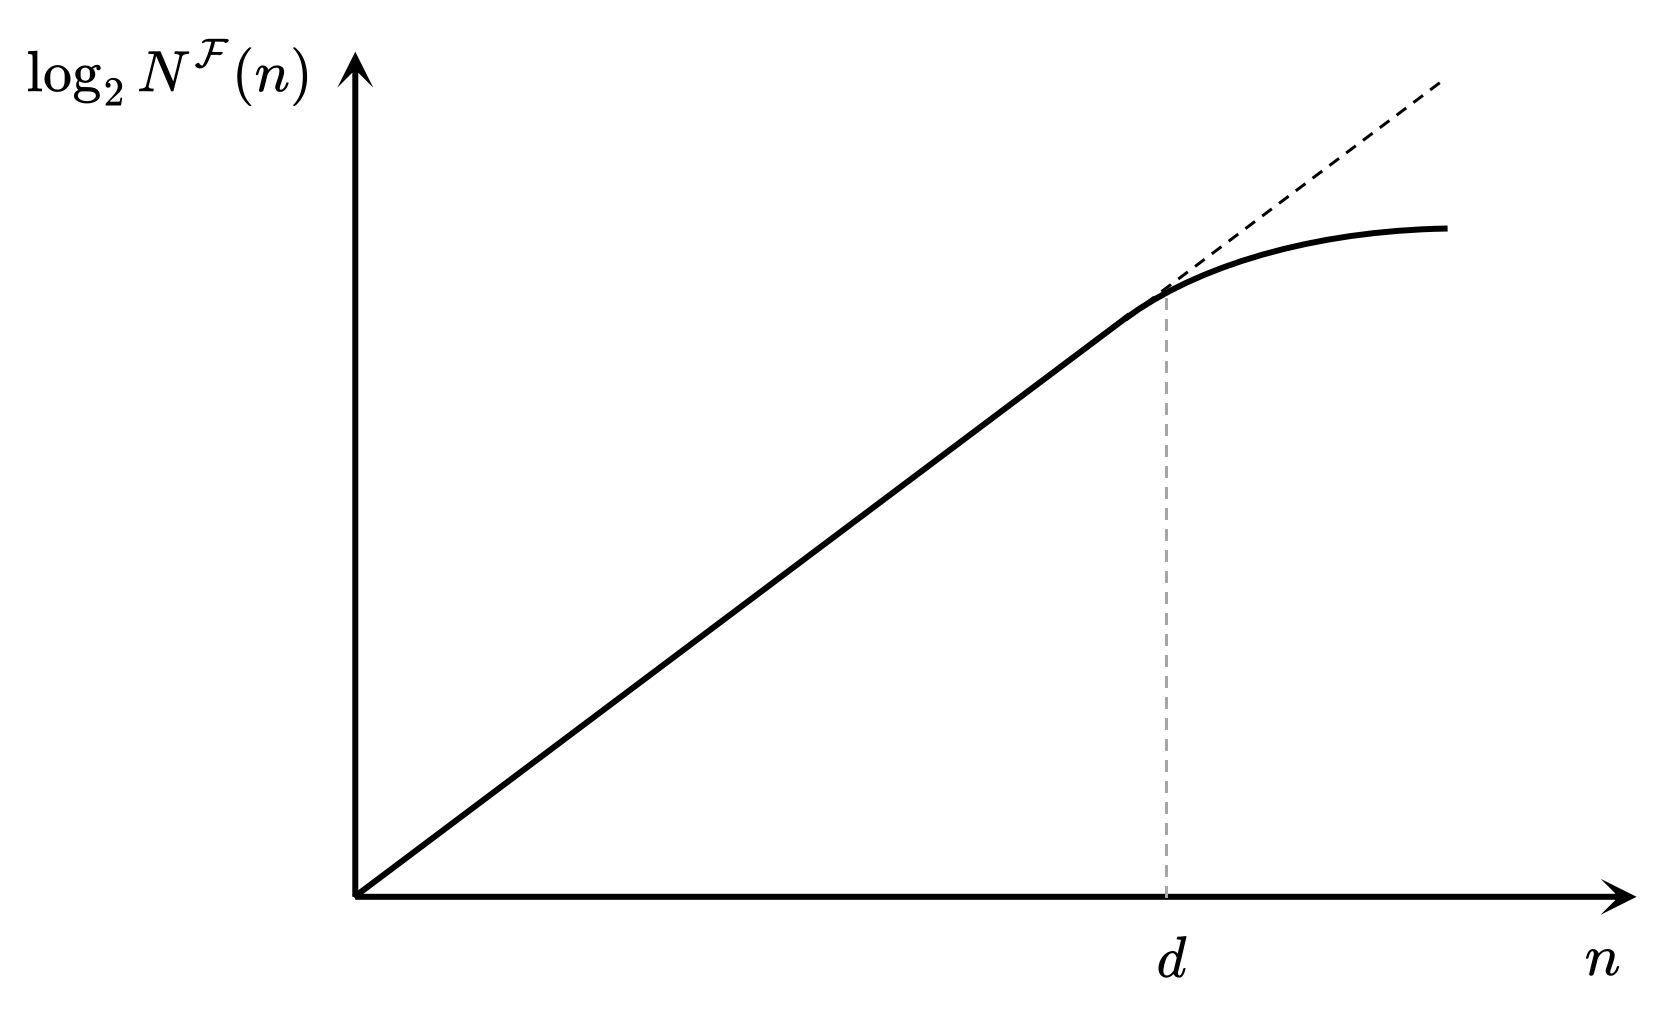
\includegraphics[width=.7\textwidth]{pic/C2_vc-dimension.png}
\end{figure} 

我们设$d$是使得$N^{\ca F}(n) = 2^n$成立的$n$的上确界. 现在想要对于$n>d$给出$N^{\ca F}(n)$的一个上界. 我们可以不妨考虑$0^{d+1}$不能被取到的情况,直接得到以下命题(至于为什么可以如此不妨假设,等待之后详细补充,现暂时留作思考)
\begin{proposition}
    对于$n > d$,有 
    \[
    N^{\ca F}(n) \le \sum_{k=0}^{d} \binom{n}{k} = \ca{O}(n^d)
    \]
\end{proposition}

下面正式给出VC维度的定义
\begin{definition} (VC维度)
    
\end{definition}

\appendix
\renewcommand{\thetheorem}{\thechapter.\arabic{theorem}}

\chapter{作业题目及解答} \label{chap:homework}

% ----- HW 1 -----

\begin{exercise} 
已知随机变量$X \sim \mathcal{N}(0, 1)$,定义 
\[
\Phi(t) := \Pr[X \ge t] = \dfrac{1}{\sqrt{2\pi}}\int_{t}^{+\infty} e^{-\tau^2/2} \dx[\tau]
\]
可以证明$\Phi$并不是初等函数,现求一个初等函数$f \sim \Phi$,即二者渐进等价。
\end{exercise}

\textbf{分析} \quad 先分析一下这个问题:显然$\Phi(t) \ra 0$,所以要$f \ra 0$. 现在$\Phi$的形式非初等不便于分析,不妨考虑$\Phi'(t) = \varphi(t)$,为此可以运用L'Hospital法则:
\[
\lim_{t \ra +\infty} \dfrac{\Phi(t)}{f(t)} = \lim_{t \ra +\infty} \dfrac{\Phi'(t)}{f'(t)} = \lim_{t \ra +\infty} \dfrac{-C e^{-t^2/2}}{f'(t)}
\]
其中$C$是某常数. 我们希望$f \sim \Phi$,也就是上述极限为1, 所以为了化简,我们希望$f'(t)$中也出现$e^{-t^2/2}$的形式. 回忆到 
\[
v(x)e^{u(x)} = \Big(v'(x) + u'(x)v(x) \Big) \cdot e^{u(x)}
\]
因此我们不妨设$f(t)$形如$g(t) e^{-t^2/2}$,此时
\[
\lim_{t \ra +\infty} \dfrac{-C e^{-t^2/2}}{f'(t)}
= \lim_{t \ra +\infty} \dfrac{-C e^{-t^2/2}}{\big[g'(t) - tg(t)\big] \cdot e^{-t^2/2}} = \lim_{t \ra +\infty}\dfrac{-C}{g'(t) - tg(t)}
\]
欲使上式为1,就要
\[
\lim_{t\ra +\infty}  tg(t) - g'(t) = \dfrac{1}{C}
\]
简便起见只考虑$C=1$,之后再给$g$乘上系数. 注意!这里千万不要把其当作$-g'(t) + tg(t) = 1$这样的一阶线性常微分方程求解,因为其解不保证初等. 如果你尝试求解ODE会发现解得$f = \Phi$确实不初等. 在这里,我们只需要考虑到$t \ra +\infty$,所以我们令$g(t) = t^{-1}$即合意.

\begin{solution}
构造初等函数 
\[
f(t) = \dfrac{1}{\sqrt{2\pi}} \cdot \dfrac{e^{-t^2/2}}{t}
\]
根据L'Hospital法则,可以验证
\[
\lim_{t\ra +\infty} \dfrac{\Phi(t)}{f(t)} = \lim_{t \ra +\infty} \dfrac{\Phi'(t)}{f'(t)} = \lim_{t \ra +\infty} \dfrac{-e^{-t^2/2}}{\left(-\dfrac{1}{t^2} - t\cdot \dfrac{1}{t}\right) e^{-t^2/2}} = \lim_{t\ra \infty}\dfrac{1+t^2}{t^2} = 1
\]
因此$f$和$\Phi$渐进等价. 
\end{solution}

事实上,我们上面给出的是 Mills 渐近展开的首项,完整的是:
\[
\Phi(t) \sim \dfrac{1}{\sqrt{2\pi}} \cdot {e^{-\frac{t^2}{2}}}
\cdot \left(
    \dfrac{1}{t} - \dfrac{1}{t^3} + \dfrac{1 \cdot 3}{x^5} - \dfrac{1 \cdot 3 \cdot 5}{x^7} + \cdots
\right)
\]

% ----- HW 2 ------

\begin{exercise}
    记 
    \[
    \ca F = \left\{
        \mathrm{sgn}(\bd{w}^{\top}\cdot \bd{x} + b): \bd{w}\in \R^d, b\in \R 
    \right\}
    \]
    其中$\mathrm{sgn}(\cdot)$是符号函数,定义为 
    \[
    \mathrm{sgn}(z) = \begin{cases}
    1 & ,z > 0\\
    -1 & ,z \le 0
    \end{cases}
    \]

    试证明:$\ca F$的VC维度是$d+1$.
\end{exercise}

\begin{proof}
记$f_{\bd{w}, b}(\bd{x}) = \mathrm{sgn}(\bd{w}^\top \cdot \bd{x} + b) \in \ca F$. 我们分两部分来证明:
\begin{enumerate}
    \item[\Circled{1}] 现取一组$\bd{x}_1, \dots, \bd{x}_{d+1}$使得其可以在$\ca F$下取到任意$d+1$维比特串. 令
    \begin{align*}
        \bd{x}_1 & = {(1, 0, \dots, 0, 0)}^\top \\
        \bd{x}_2 & = {(0, 1, \dots, 0, 0)}^\top \\
                & \vdots \\
        \bd{x}_d & = {(0, 0, \dots, 0, 1)}^\top \\
        \bd{x}_{d+1} & = {(0, 0, \dots, 0, 0)}^\top
    \end{align*}
    
    那么对于任意的$\bd{y} = (y_1, \dots, y_{d+1}) \in \{\pm 1\}^{d+1}$,取 
    \[
    \bd{w}_0 = 2\bd{y}_{1:d}^\top = {(2y_1, \dots, 2y_{d})}^\top, \quad b_0 = y_{d+1}
    \]

    则由于$\bd{y}$的各个元素取值于$\{\pm 1\}$,不难证明
    \begin{align*}
        f_{\bd{w}_0, b_0}(\bd{x}_j) & = \mathrm{sgn}(\bd{w}_0^\top \bd{x}_j+ b_0) = \mathrm{sgn}(2y_j + y_{d+1}) = y_j &, j=1,\dots,d \\
        f_{\bd{w}_0, b_0}(\bd{x}_{d+1}) & = \mathrm{sgn}(\bd{w}_0^\top \bd{0}+ b_0) = \mathrm{sgn}(y_{d+1}) = y_{d+1}
    \end{align*}
    
    至此我们说明对于任意$d+1$维比特串,都存在$f\in \ca F$使得$(\bd{x}_1, \dots, \bd{x}_{d+1})$在$f$的像是该比特串. 

    \item[\Circled{2}] 对于任意$\bd{x}_1, \dots, \bd{x}_{d+2}$,往证明一定有其取不到的比特串. 我们令$\tilde{\bd{x}}_j = {(\bd{x}_j^\top, 1)}^\top \in \R^{d+1}$(即添加一个1)那么根据向量空间基本定理可知这些向量线性相关,即存在一组不全为零的实数$\ld_1, \dots, \ld_{d+2}$使得 
    \[
    \sum_{j=1}^{d+2} \ld_j \cdot \tilde{\bd{x}}_j = \bd{0} \quad \Ra \quad \sum_{j=1}^{d+2} \ld_j \cdot \bd{x}_j = \sum_{j=1}^{d+2} \ld_j = 0
    \]

    现在任取$\bd{w}\in \R^d, b\in \R$,我们知道 
    \begin{equation} \label{eq:hw2-1}
    \sum_{j=1}^{d+1} \ld_j \cdot \big(\bd{w}^{\top}\bd{x}_j + b\big) = b \cdot \sum_{j=1}^{d+1} \ld_j = 0
    \end{equation}

    因此我们可以断言
    \[
    \big(
        f_{\bd{w}, b}(\bd{x}_1), \dots, f_{\bd{w}, b}(\bd{x}_{d+2})
    \big) \neq \big(
        \mathrm{sgn}(\ld_1), \dots, \mathrm{sgn}(\ld_{d+2})
    \big)
    \]

    否则\hyperref[eq:hw2-1]{A.1式}左侧与$\sum_j \abs{\ld_j}$同号,而这是正数$>0$会导致矛盾.
    
    至此我们说明了一定存在取不到的$d+2$维比特串.
    
\end{enumerate}
综上所述,我们证明了$\ca F$的VC维度是$d+1$.
\end{proof}
\chapter{学期课题} 
\chapter{往年题选及解答}

\end{document}